    \documentclass[12pt]{article}
    \usepackage{amsmath}
    \usepackage{graphicx}
    \usepackage{multirow}
    \usepackage{booktabs}
    \usepackage{subfigure}
    \usepackage{verbatim}
    \usepackage{color}
    \usepackage{hyperref}
    \usepackage{url}
    \usepackage{axessibility} 
    
    
    \begin{document}

    \title{PHYS131 -- IT Skills -- Worksheet 4}
    \author{Samuel Hedges}
    \date{\today}
    \maketitle

    \begin{abstract}
    This is my second document typeset in \LaTeX.\\ \textit{I declare that this submission is my own work. I have not submitted it in substantially the same form towards the award of a degree or other qualification. It has not been written or composed by any other person and all sources have been referenced or acknowledged.}
    \end{abstract}

    \tableofcontents

\section{Introduction}

In addition to the Introduction and the Summary sections, this document contains three other sections:  Table in colours, Sec. \ref{sec:TabCol},  Figures, Sec. \ref{sec:Figs} and Some Feynman's works, Sec. \ref{sec:Feynman}.

\section{A table in colours}
\label{sec:TabCol}
\begin{center}
    \begin{tabular}{|c|c|}
    \hline
\color{white} \colorbox{red}{Equation}  &\color{white} \colorbox{blue}{Solution} \\ \hline
\color{red} $ax + b = 0$ &\color{blue} $x = -b/a$\\ \hline
\color{red} \multirow {5}{*}{$ax^{2} + bx + c = 0$} &\\ 
 &\color{blue}$x_{1} = \frac{-b + \sqrt{b^{2}-4ac}}{2a}$ \\
& \\
 &\color{blue}$x_{2} = \frac{-b - \sqrt{b^{2}-4ac}}{2a}$\\
&\\ \hline

    \end{tabular}
    \\\textbf{Table 1: Two equations and their solution in a colourful table}
\end{center}


\section{Figures}
\label{sec:Figs}

This section contains figures
\\
\begin{figure}[!ht]
    \centering
    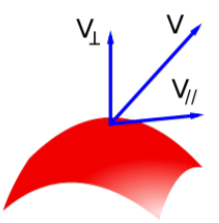
\includegraphics[scale=0.5]{week 4/Diagram.png}
    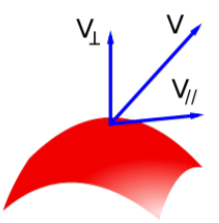
\includegraphics[angle=45,scale=0.5]{week 4/Diagram.png}
    \caption{Illustration of tangential and normal components of a vector to a surface. The figure is presented in its original form (left) and rotated (right)}
    \label{fig:my_label}
\end{figure}



\section{Some Feynman's works}
\label{sec:Feynman}
Richard Phillips Feynman %(Fig. \ref{Fig:Feynman})
was an American theoretical physicist known for his work in the path integral formulation of quantum mechanics, the theory of quantum electrodynamics, and the physics of the superfluidity of supercooled liquid helium, as well as in particle physics for which he proposed the parton model. For his contributions to the development of quantum electrodynamics, Feynman, jointly with Julian Schwinger and Sin-Itiro Tomonaga, received the Nobel Prize in Physics in 1965. For further details see \url{https://en.wikipedia.org/wiki/Richard_Feynman}.


\begin{figure}[h!]
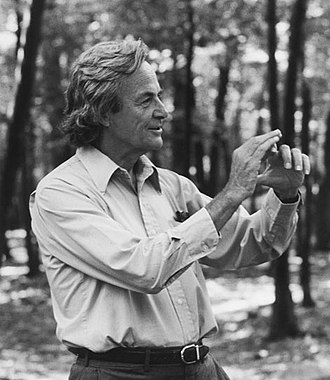
\includegraphics[scale=0.3]{Richard F.jpg}
\caption{ Richard Feynman at the Robert Treat Paine Estate in Waltham, Massachusetts, in 1984. }
\label{fig:Feynman}
\end{figure}

Faynman's works include --

\begin{itemize}
\item Scientific works; 3 of which are listed below (\cite{Feynman:48a}--\cite{Feynman:48c}),
\item Textbooks and lecture notes; 2 of which are included below (\cite{Feynman:61,Feynman:62}),
\item Popular works. Two of them, {\em Surely You're Joking, Mr. Feynman!: Adventures of a Curious Character} and {\em ``What Do You Care What Other People Think?'': Further Adventures of a Curious Character},  are listed below (\cite{Feynman:85,Feynman:88}).
\end{itemize}



\section{Summary}

I have created a complex document in \LaTeX. It contains a colored table, figures and bibliographic data.\\

\text{ All seven of these books can be found at Lancaster University Library.}\\

\text{ \cite{Feynman:61, Feynman:62, Feynman:85, Feynman:88} can be found in hard copy at Lancaster University Library}

\begin{thebibliography}{99}
\bibitem{Feynman:48a} Feynman, Richard P. (1948), ``Space-time approach to non-relativistic quantum mechanics'', {\em Reviews of Modern Physics} {\bf 20}(2): 367–-387.
\bibitem{Feynman:48b} Feynman, Richard P. (1948). "A Relativistic Cut-Off for Classical Electrodynamics". Physical Review. 74 (8):939-946
\bibitem{Feynman:48c} Feynman, Richard P. (1948). "Relativistic Cut-Off for Quantum Electrodynamics". Physical Review. 74 (10): 1430–1438.
\bibitem{Feynman:61} Feynman, Richard P. (1961), {\em Theory of Fundamental Processes}, Addison Wesley.
\bibitem{Feynman:62} Feynman, Richard P. (1962). Quantum Electrodynamics. Addison Wesley.
\bibitem{Feynman:85} Feynman, Richard P. and Ralph Leighton (1985),  {\em Surely You're Joking, Mr. Feynman!: Adventures of a Curious Character}, W. W. Norton \& Co.
\bibitem{Feynman:88}Feynman, Richard P. and Ralph Leighton (1988),  {\em What Do You Care What Other People Think?": Further Adventures of a Curious Character}, W. W. Norton \& Co

\end{thebibliography}


    \end{document}
